% Generated by make_thesis_pgfplots.py -- do not edit by hand.
\definecolor{vizblue}{HTML}{2A78D6}
\definecolor{vizorange}{HTML}{EB6834}
\definecolor{vizaqua}{HTML}{1BAF7A}
\definecolor{vizgrid}{HTML}{E1E0D9}
\definecolor{vizaxis}{HTML}{C3C2B7}
\definecolor{vizmuted}{HTML}{898781}
\definecolor{vizink}{HTML}{52514E}

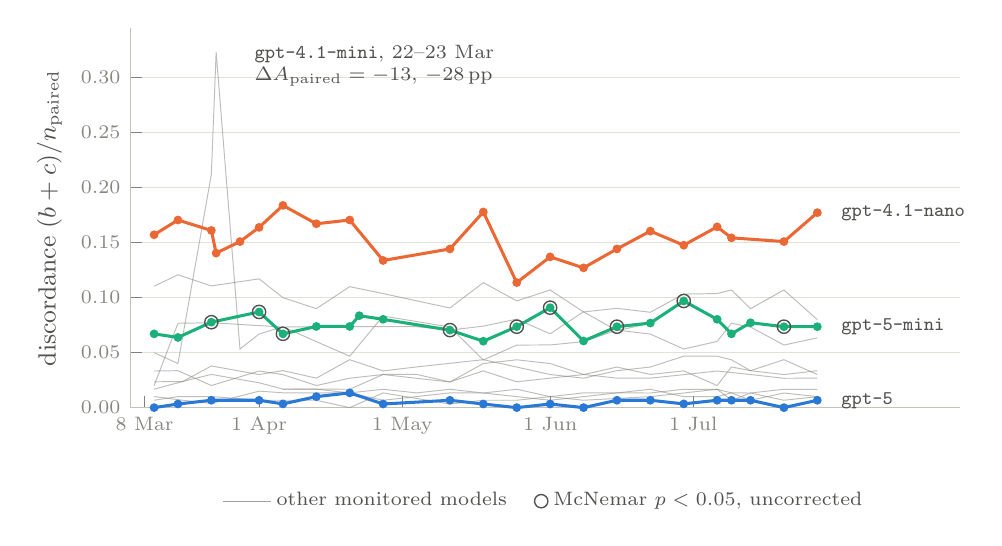
\begin{tikzpicture}
    \begin{axis}[
        width=\linewidth, height=6.4cm,
        xmin=-3, xmax=171, ymin=0, ymax=0.345,
        xtick={0,24,54,85,115},
        xticklabels={8 Mar,1 Apr,1 May,1 Jun,1 Jul},
        ytick={0,0.05,0.10,0.15,0.20,0.25,0.30},
        yticklabel style={/pgf/number format/fixed, /pgf/number format/fixed zerofill, /pgf/number format/precision=2},
        ylabel={discordance $(b+c)/n_{\mathrm{paired}}$},
        legend columns=2,
        legend style={at={(0.5,-0.20)}, anchor=north, /tikz/every even column/.append style={column sep=8pt}},
        axis line style={vizaxis, line width=0.4pt},
        tick label style={vizmuted, font=\scriptsize},
        label style={vizink, font=\small},
        legend style={draw=none, fill=none, font=\scriptsize,
                      text=vizink, inner sep=1pt},
        grid=major,
        grid style={vizgrid, line width=0.4pt},
        axis x line*=bottom,
        axis y line*=left,
        ymajorgrids=true,
        xmajorgrids=false,
        clip=false,
    ]
    \addplot[vizmuted, line width=0.35pt, opacity=0.55, forget plot] coordinates {(2,0.0168) (8,0.0238) (14,0.0302) (24,0.0226) (29,0.0169) (36,0.0168) (43,0.0167) (50,0.0302) (57,0.0302) (64,0.0234) (71,0.0334) (78,0.0235) (85,0.0268) (92,0.0301) (99,0.0369) (106,0.0302) (113,0.0334) (120,0.0201) (123,0.0370) (127,0.0336) (134,0.0301) (141,0.0336)};
    \addplot[vizmuted, line width=0.35pt, opacity=0.55, forget plot] coordinates {(2,0.0235) (8,0.0237) (14,0.0379) (24,0.0301) (29,0.0337) (36,0.0268) (43,0.0436) (50,0.0334) (57,0.0370) (64,0.0403) (71,0.0436) (78,0.0369) (85,0.0301) (92,0.0268) (99,0.0336) (106,0.0369) (113,0.0468) (120,0.0468) (123,0.0435) (127,0.0336) (134,0.0436) (141,0.0301)};
    \addplot[vizmuted, line width=0.35pt, opacity=0.55, forget plot] coordinates {(2,0.0101) (8,0.0067) (14,0.0038) (24,0.0150) (29,0.0135) (36,0.0134) (43,0.0134) (50,0.0167) (57,0.0134) (64,0.0167) (71,0.0133) (78,0.0100) (85,0.0067) (92,0.0100) (99,0.0134) (106,0.0167) (113,0.0100) (120,0.0100) (123,0.0134) (127,0.0067) (134,0.0133) (141,0.0100)};
    \addplot[vizmuted, line width=0.35pt, opacity=0.55, forget plot] coordinates {(2,0.0200) (7,0.0767) (14,0.0772) (29,0.0733) (36,0.0736) (43,0.0736) (57,0.0736) (64,0.0705) (71,0.0741) (78,0.0805) (85,0.0671) (92,0.0872) (99,0.0700) (106,0.0767)};
    \addplot[vizmuted, line width=0.35pt, opacity=0.55, forget plot] coordinates {(2,0.0500) (7,0.0401) (14,0.2121) (15,0.3233) (20,0.0533) (24,0.0669) (29,0.0736) (36,0.0600) (43,0.0468) (50,0.0833) (64,0.0733) (71,0.0433) (78,0.0569) (85,0.0570) (92,0.0600) (99,0.0705) (106,0.0669) (113,0.0533) (120,0.0602) (123,0.0767) (127,0.0733) (134,0.0569) (141,0.0635)};
    \addplot[vizmuted, line width=0.35pt, opacity=0.55, forget plot] coordinates {(2,0.1104) (7,0.1208) (14,0.1107) (24,0.1171) (29,0.1000) (36,0.0900) (43,0.1100) (50,0.1037) (64,0.0906) (71,0.1137) (78,0.0970) (85,0.1070) (92,0.0870) (99,0.0903) (106,0.0867) (113,0.1033) (120,0.1037) (123,0.1070) (127,0.0900) (134,0.1070) (141,0.0800)};
    \addplot[vizmuted, line width=0.35pt, opacity=0.55, forget plot] coordinates {(2,0.0333) (7,0.0336) (14,0.0201) (24,0.0333) (29,0.0300) (36,0.0201) (43,0.0268) (50,0.0301) (64,0.0233) (71,0.0401) (78,0.0435) (85,0.0401) (92,0.0302) (99,0.0268) (106,0.0268) (113,0.0300) (120,0.0333) (127,0.0301) (134,0.0267) (141,0.0268)};
    \addplot[vizmuted, line width=0.35pt, opacity=0.55, forget plot] coordinates {(2,0.0067) (7,0.0100) (14,0.0101) (24,0.0067) (29,0.0067) (36,0.0067) (43,0.0000) (50,0.0134) (64,0.0033) (71,0.0067) (78,0.0067) (85,0.0100) (92,0.0067) (106,0.0100) (113,0.0133) (120,0.0167) (123,0.0134) (127,0.0133) (134,0.0067) (141,0.0100)};
    \addplot[vizmuted, line width=0.35pt, opacity=0.55, forget plot] coordinates {(29,0.0167) (36,0.0168) (43,0.0134) (50,0.0067) (64,0.0134) (71,0.0133) (78,0.0167) (85,0.0100) (92,0.0134) (99,0.0134) (106,0.0133) (113,0.0167) (120,0.0167) (123,0.0067) (127,0.0133) (134,0.0167) (141,0.0167)};
    \addplot[vizorange, line width=1.1pt, mark=*, mark size=1.0pt, mark options={fill=vizorange, draw=vizorange}, forget plot] coordinates {(2,0.1572) (7,0.1706) (14,0.1611) (15,0.1405) (20,0.1510) (24,0.1639) (29,0.1839) (36,0.1672) (43,0.1706) (50,0.1338) (64,0.1443) (71,0.1779) (78,0.1137) (85,0.1371) (92,0.1271) (99,0.1443) (106,0.1605) (113,0.1477) (120,0.1644) (123,0.1544) (134,0.1510) (141,0.1773)};
    \node[anchor=west, font=\scriptsize, text=vizink] at (axis cs:144,0.1773) {\texttt{gpt-4.1-nano}};
    \addplot[vizaqua, line width=1.1pt, mark=*, mark size=1.0pt, mark options={fill=vizaqua, draw=vizaqua}, forget plot] coordinates {(2,0.0671) (7,0.0638) (14,0.0777) (24,0.0870) (29,0.0671) (36,0.0738) (43,0.0738) (45,0.0836) (50,0.0803) (64,0.0705) (71,0.0604) (78,0.0736) (85,0.0909) (92,0.0606) (99,0.0736) (106,0.0769) (113,0.0970) (120,0.0803) (123,0.0671) (127,0.0772) (134,0.0736) (141,0.0736)};
    \node[anchor=west, font=\scriptsize, text=vizink] at (axis cs:144,0.0736) {\texttt{gpt-5-mini}};
    \addplot[vizblue, line width=1.1pt, mark=*, mark size=1.0pt, mark options={fill=vizblue, draw=vizblue}, forget plot] coordinates {(2,0.0000) (7,0.0033) (14,0.0067) (24,0.0067) (29,0.0034) (36,0.0100) (43,0.0134) (50,0.0033) (64,0.0067) (71,0.0033) (78,0.0000) (85,0.0033) (92,0.0000) (99,0.0067) (106,0.0067) (113,0.0034) (120,0.0067) (123,0.0067) (127,0.0067) (134,0.0000) (141,0.0067)};
    \node[anchor=west, font=\scriptsize, text=vizink] at (axis cs:144,0.0067) {\texttt{gpt-5}};
    \addplot[only marks, mark=o, mark size=2.4pt, draw=vizink, line width=0.5pt, forget plot] coordinates {(14,0.0777) (24,0.0870) (29,0.0671) (64,0.0705) (78,0.0736) (85,0.0909) (99,0.0736) (113,0.0970) (134,0.0736)};
    \addlegendimage{vizmuted, line width=0.35pt, opacity=0.8}
    \addlegendentry{other monitored models}
    \addlegendimage{only marks, mark=o, mark size=2.4pt, draw=vizink, line width=0.5pt}
    \addlegendentry{McNemar $p<0.05$, uncorrected}
    \node[anchor=west, font=\scriptsize, text=vizink, align=left] at (axis cs:21,0.3113) {\texttt{gpt-4.1-mini}, 22--23~Mar\\$\Delta A_{\mathrm{paired}}=-13$, $-28$\,pp};
    \end{axis}
\end{tikzpicture}
